% Source: AESP_466_ClassWork/Exams/Midterm/AESP466_Midterm_StudyGuide_Addendum_Sp26.tex

\documentclass[border=4pt]{standalone}
\usepackage{amsmath}
\usepackage{amssymb}
\usepackage{graphicx}
\usepackage{tikz}
\usepackage{xcolor}

\definecolor{Garnet}{HTML}{73000A}
\definecolor{USC_Rose}{HTML}{CC2E40}
\definecolor{USC_Blue}{HTML}{466A9F}
\definecolor{USC_Slate}{HTML}{1F414D}
\definecolor{USC_Olive}{HTML}{65780B}
\definecolor{USC_Black90}{HTML}{565656}
\definecolor{USC_Black10}{HTML}{ECECEC}

\begin{document}
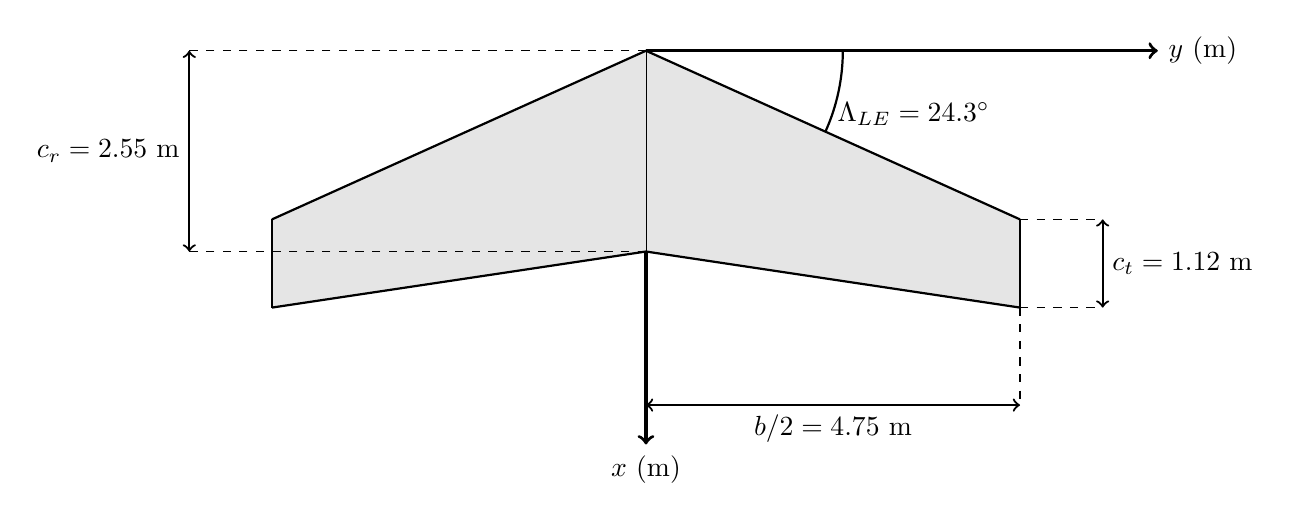
\begin{tikzpicture}[scale=1.0]
% Coordinate system at wing apex (LE of root)
\draw[->, very thick] (0,0) -- (0,-5) node[below] {$x$ (m)};
\draw[->, very thick] (0,0) -- (6.5,0) node[right] {$y$ (m)};
% Right half-wing: c_r=2.55, c_t=1.12, b/2=4.75, sweep=24.3 deg
% LE tip x-offset = 4.75*tan(24.3) = 2.142
\fill[gray!20] (0,0) -- (4.75,-2.142) -- (4.75,-3.262) -- (0,-2.55) -- cycle;
\draw[thick] (0,0) -- (4.75,-2.142);          % Leading edge
\draw[thick] (0,-2.55) -- (4.75,-3.262);      % Trailing edge
\draw[thick] (0,0) -- (0,-2.55);              % Root chord
\draw[thick] (4.75,-2.142) -- (4.75,-3.262);  % Tip chord
% Left half-wing (mirror)
\fill[gray!20] (0,0) -- (-4.75,-2.142) -- (-4.75,-3.262) -- (0,-2.55) -- cycle;
\draw[thick] (0,0) -- (-4.75,-2.142);
\draw[thick] (0,-2.55) -- (-4.75,-3.262);
\draw[thick] (-4.75,-2.142) -- (-4.75,-3.262);
% Dimension: root chord
\draw[dashed, thin] (0,0) -- (-5.8,0);
\draw[dashed, thin] (0,-2.55) -- (-5.8,-2.55);
\draw[<->, thick] (-5.8,0) -- (-5.8,-2.55);
\node[left] at (-5.8,-1.275) {$c_r = 2.55$ m};
% Dimension: tip chord
\draw[dashed, thin] (4.75,-2.142) -- (5.8,-2.142);
\draw[dashed, thin] (4.75,-3.262) -- (5.8,-3.262);
\draw[<->, thick] (5.8,-2.142) -- (5.8,-3.262);
\node[right] at (5.8,-2.702) {$c_t = 1.12$ m};
% Dimension: semi-span
\draw[dashed, thin] (0,-3.262) -- (0,-4.5);
\draw[dashed, thin] (4.75,-3.262) -- (4.75,-4.5);
\draw[<->, thick] (0,-4.5) -- (4.75,-4.5);
\node[below] at (2.375,-4.5) {$b/2 = 4.75$ m};
% Sweep angle arc
\draw[dashed] (0,0) -- (3.5,0);
\draw[thick] (2.5,0) arc (0:-24.3:2.5);
\node at (3.4,-0.8) {$\Lambda_{LE} = 24.3^\circ$};
\end{tikzpicture}
\end{document}
